\level{2}{ASpeedControllerFromTriacTrigger}

\level{3}{Structure}
{
\centering{}
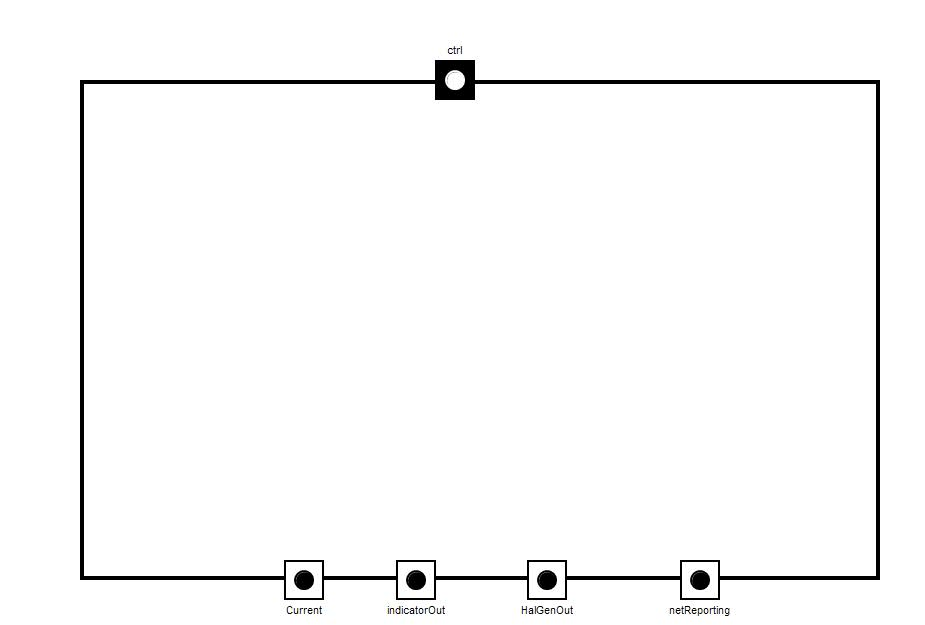
\includegraphics[width=1.0\textwidth]{./images/ASpeedControllerFromTriacTrigger_structure.jpg}
\figcaption{ASpeedControllerFromTriacTrigger Structure}
}

\level{3}{Ports}
\begin{tabular}[ht]{|l|l|l|l|l|p{5cm}|}
\hline
\textbf{Name} & \textbf{Protocol} & \textbf{Type} & \textbf{Kind} & \textbf{Multiplicity} & \textbf{Description}\\
\hline
HalGenOut & PSpeed & conj. & external & 1 & \\
\hline
indicatorOut & POnOff & conj. & external & 1 & \\
\hline
Current & PDacIntern & conj. & external & 1 & \\
\hline
ctrl & PSpeedControllerFromPwmCtrl & reg. & external & 1 & \\
\hline
netReporting & PNetClockReport & conj. & external & 1 & \\
\hline
\end{tabular}

\level{3}{Behavior}
\level{4}{Top Level}
{
\centering{}
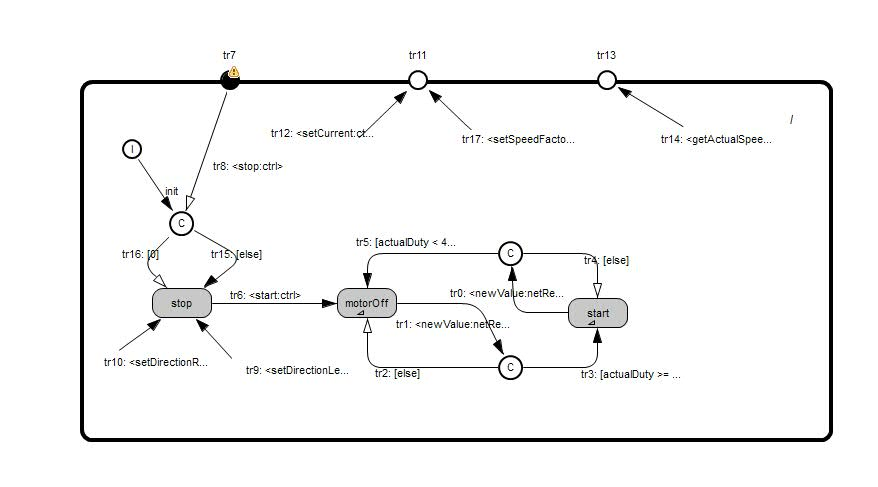
\includegraphics[width=1.0\textwidth]{./images/ASpeedControllerFromTriacTrigger_behavior.jpg}
\figcaption{ASpeedControllerFromTriacTrigger Top State}
}

\begin{par}

\end{par}


\level{3}{Attributes}
\begin{tabular}[ht]{|l|l|p{8cm}|}
\hline
\textbf{Name} & \textbf{Type} & \textbf{Description}\\
\hline
actualSpeed & uint32 & \\
\hline
oldSpeed & uint32 & \\
\hline
actualDuty & uint32 & % begin text from user Documentation
0..100 => 0..100%
% end text from user Documentation
\\
\hline
speedFactor & uint32 & \\
\hline
maxSpeedStep & uint32 & \\
\hline
\end{tabular}

\level{3}{Operations}
\begin{tabular}[ht]{|l|l|}
\hline		
	Name: & calcActualSpeed\\
	\hline
	ReturnType: &  void\\
	\hline
	Arguments: & \\
	\hline
\end{tabular}
\newline\newline\newline
